% !TEX root = /media/ueslei/Ueslei/INPE/PCI/Projetos/Guia_COAWST/main.tex
\chapterimage{header.jpg}
\chapter{Building the weights between grids with SCRIP}
\bigskip
\section{Building the weights}
\bigskip
\noindent As seen in the section \textcolor{bleu_cite}{\ref{scripsecao}}, SCRIP is used to interpolate the weights between two or more grids of different models. 
In COAWST, the package was modified to generate only one NetCDF file that will be used during integrations.
\bigskip

\noindent The SCRIP directory is located at:
\bigskip

\begin{bashcode}
/home/name.surname/COAWST/Lib/SCRIP
\end{bashcode}
\bigskip

\noindent Inside the folder, look for the file with the extension\textit{.in}. As in the example in Figure \textcolor{bleu_cite}{\ref{scripinnedit}}:

\begin{figure}[H]
    \centering
    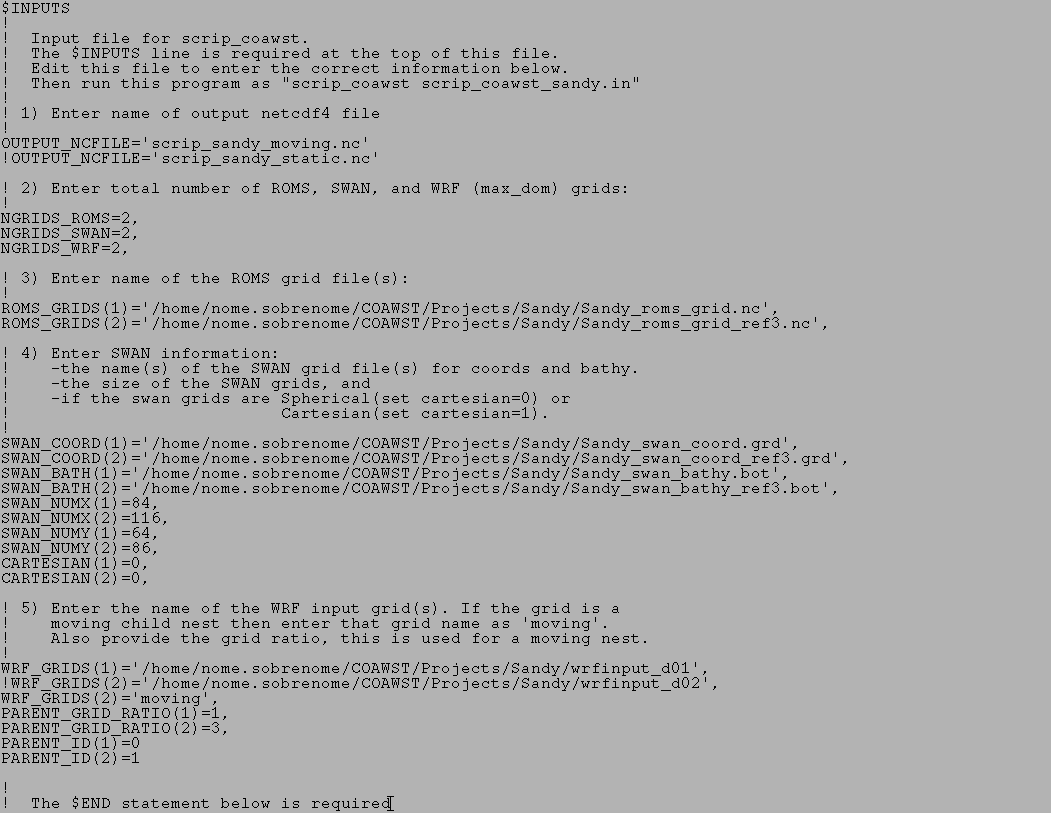
\includegraphics[width=0.65\textwidth]{scripin.png}
    \caption{SCRIP \textit{.in} file for the Sandy project.}
    \label{scripinnedit}
\end{figure}
\bigskip

\noindent In \textit{OUTPUT\_NCFILE}, change the name of the NetCDF file that will be generated if necessary.
\bigskip

\noindent In section 2 of the file, change the variables \textit{NGRIDS\_ROMS}, \textit{NGRIDS\_SWAN} and \textit{NGRIDS\_WRF} according to the number of grids, 
existing in your project, in ROMS, SWAN and WRF, respectively.
\bigskip

\noindent In the third section of the file, renew the ROMS grid directories according to the names in your project.
\bigskip

\noindent For SWAN, in the fourth section, in addition to changing the directories of the SWAN grids (\textit{SWAN\_COORD} and \textit{SWAN\_BATH}), change the 
number of existing grid points, according to your project , in the variables \textit {SWAN\_NUMX} and \textit{SWAN\_NUMY}.
\bigskip

\noindent Finally, in the fifth section, change the WRF grid directories (\textit{WRF\_GRIDS}). In \textit {PARENT\_GRID\_RATIO}, if your project includes nesting 
between the WRF grids, change to the relationship used between the grids used in your project. In \textit{PARENT\_ID}, add the grid ID.
\bigskip

\noindent Then, save the changes.
\bigskip

\noindent To run SCRIP, search the repository for the file \textit{qsub\_scrip.sh}:
\bigskip

\begin{bashcode}
/home/name.surname/repositorio/qsub_scrip.sh
\end{bashcode}
\bigskip

\noindent Move the file to the SCRIP directory:
\bigskip

\begin{bashcode}[fontsize=\scriptsize]
mv /home/name.surname/repositorio/qsub_scrip.sh /home/name.surname/COAWST/Lib/SCRIP
\end{bashcode}
\bigskip

\noindent Open the file \textit{qsub\_scrip.sh}:
\bigskip

\begin{bashcode}
nedit qsub_scrip.sh
\end{bashcode}
\bigskip

\noindent Change and save the file \textit{.sh}, as in the example in Figure \textcolor{bleu_cite}{\ref{qsubscripsh}}:
\bigskip

\begin{figure}[H]
    \centering
    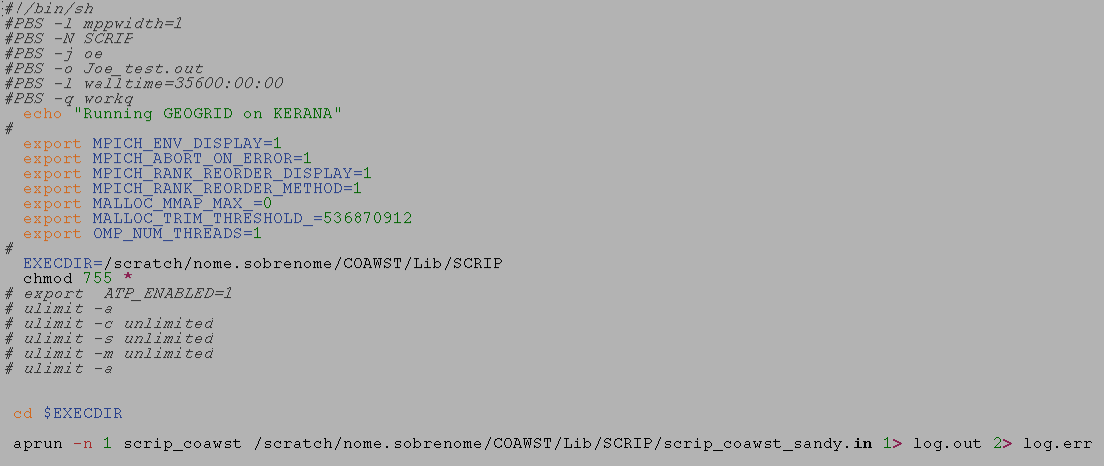
\includegraphics[width=0.65\textwidth]{scripqsub.png}
    \caption{\textit{.sh} file used to run SCRIP.}
    \label{qsubscripsh}
\end{figure}
\bigskip

\noindent To start SCRIP, type:
\bigskip

\begin{bashcode}
qsub qsub_scrip.sh
\end{bashcode}
\bigskip

\noindent At the end, the file \textit{scrip\_static.nc} will be created. Now put them in your project folder and you're done! COAWST is ready to run.
\bigskip

\section{Executing your project}{{{{ }}}}
\bigskip

\noindent Now, with everything ready, your project is ready to be executed. Visit the section \textcolor{bleu_cite}{\ref{sandyexec}} to remember 
how to execute the project.